	

    \documentclass[a4paper,11pt]{article}
     
    \usepackage[english]{babel}
    \usepackage[utf8x]{inputenc}
    \usepackage{graphicx}
    \usepackage{geometry}
    \geometry{
            body={170mm,230mm},
            left=25mm,top=25mm,
            headheight=25mm,headsep=7mm,
            marginparsep=4mm,
            marginparwidth=20mm,
            footnotesep=50mm
    }
    \usepackage{enumitem}
    \setlist{noitemsep}
    \usepackage{amsmath}
     
    \title{INFO-F-404: Real-Time Operating Systems\\2013 -- 2014 Project 1: Least Laxity First}
    \author{\textsc{Delhaye} Quentin}
     
    \begin{document}
    \maketitle
    \section{Implementation}
    \subsection{Task Generator}
    The \texttt{main} function of \texttt{taskGenerator} does the following:
    \begin{itemize}
    \item parsing the program arguments;
    \item creating an \texttt{Generator} object with those arguments;
    \item asking the object to generate the tasks and saving them to a file.
    \end{itemize}
     
    The \texttt{WCET} of each task is randomly chosen in the interval $[1;30]$. Similarly, the deadline randomly chosen between the end of the \texttt{WCET} and the end of the period.
     
    Saving the tasks into a file is optional, since the analyzer will just require a table with the parameters.
     
    \subsection{LLF Scheduler}
    The \texttt{main} function of \texttt{simLLF} does the following:
    \begin{itemize}
    \item parsing the program arguments;
    \item extract the information concerning the tasks from the file given in argument;
    \item create a new object \texttt{Simulator} that will handle the rest of the job.
    \end{itemize}
     
    The simulator begins by creating an array of \texttt{Task} objects with the required parameters. The simulation can then begin, for more information about this part, please refer to the appendix~\ref{an:stateDiag}.
     
    The computation of the study interval is based on the well-known Euclidean algorithm that give the \textit{gcd} of two numbers. Knowing that $\mbox{gcd(a,b,c)} = \mbox{gcd(gcd(a,b),c)}$, the \textit{lcm} of the set is immediate.
     
    Since the system has to be scheduled following the LLF, the \texttt{setPriorities} method will ask to each to compute its own laxity, and then will sort the array containing all the tasks and their corresponding laxity.
     
    When the simulation is successful, that is if no task has ever missed its deadline, the \texttt{Simulator} class creates then a new \texttt{GraphCreator} object that will create a \texttt{png} image representing the scheduling of the system.
    This image is created using the \texttt{pngwriter} library (which should then be installed on the system).
    The points used by this object to generate the image are the begining and ending time of each job, the begining and ending type (preemption, recovery, or normal) as well as the task number (an idle time having an id = $-1$).
     
    \begin{figure}
    \centering
    
\includegraphics{tasksEDFvsLLF}
    \caption{LLF Scheduling of two tasks}
    \label{fig:tasksEDFvsLLF}
    \end{figure}
     
    As an example, the figure~\ref{fig:tasksEDFvsLLF} represents the scheduling of the system proposed in the first chapter of the course,
    slides 83 and 84, with a re-computation of the priorities each unit of time (delta $= 0$).
     
    The red triangles reprensent a preemption, the white arrows the arriving of a new job, the white diamonds the deadline, and the green area the idle time of the CPU.
     
    \subsection{LLF Analyzer}
    The analyser \texttt{LLF\_study} implements all the previous classes. It will begin by generating a set of tasks, and then will simulate them.
     
    For further details, please refer to the section~\ref{sec:anal}.
     
     
     
     
    \section{Difficulties}
    \paragraph{Split the utilization between the tasks} During the generation of the tasks based on the arguments given to \texttt{taskGenerator}, one of the difficulties was to determine what should the utilization of each task be
    in order to have the expected system utilization at the end.
    The solution chosen is the simplest: assigning the same utilization to each task.
     
    It is to be noted that due to this method and because of the use of natural numbers, the actual utilization is a bit off.
     
    \section{Simulations}\label{sec:anal}
    There are three free parameters in our system: the utilization, the number of tasks in the system, and the \textit{delta}\footnote{The \textit{delta} is the period at which the priorities are computed.}.
     
    They will be all compared to the other two, each time one parameter being fixed.
     
    \textit{Notes:} some cells will be filled with "N/A" in the case the system was not schedulable. Otherwise, each cell will contain a triplet of intergers: \{study interval, preemptions, idle time\}
     
	\subsection{Results}
    \paragraph{First round: fixed number of tasks (3), various
	\textit{delta} and utilization:~table~\ref{tb:test1}}
    \begin{table}[!h]
    \centering
    \begin{tabular}{|c|c|c|c|c|c|} \hline
       & 50 & 60 & 70 & 80 & 90 \\ \hline
			1&1008;78;519&2550;120;1172&672;20;234&N/A&N/A\\ \hline
		2&2340;52;1201&350;0;163&N/A&N/A&N/A \\ \hline
		5&N/A&29750;25;12521&780;23;212&N/A&N/A\\ \hline
		10&42120;64;21815&N/A&360;2;97&N/A&N/A \\ \hline
		20&N/A&N/A&N/A&N/A&N/A \\ \hline
   \end{tabular}
    \caption{Horizontally: \textit{delta}, vertically: utilization}
	\label{tb:test1}
    \end{table}
     
     
    \paragraph{Second round: fixed \textit{delta} (2), various number of task and utilization:~table~\ref{tb:test2}}
    \begin{table}[!h]
    \centering
    \begin{tabular}{|c|c|c|c|c|c|} \hline
       & 50 & 60 & 70 & 80 & 90 \\ \hline
		2&N/A&N/A&N/A&N/A&N/A \\ \hline
		3&5400;97;2898 & N/A & N/A & N/A & N/A \\ \hline
		5 & 75600;0;39395 & N/A & 33810;691;10731 & N/A & N/A \\ \hline
		7 & 3800160;0;2106620 & 12870;86;5336 & 46200;999;14795 & N/A & N/A \\ \hline
		9 & 249480;1573;130734&6054750;32531;2671512 & N/A & N/A & N/A \\ \hline
   \end{tabular}
    \caption{Horizontally: number of task, vertically: utilization}
	\label{tb:test2}
    \end{table}
	
	Let's note that the second ligne of the table~\ref{tb:test2} is pathologic.
     
	\paragraph{Third round: fixed utilization (70), various number of task and \textit{delta}:~table~\ref{tb:test3}}
    \begin{table}[!h]
    \centering
    \begin{tabular}{|c|c|c|c|c|c|} \hline
		& 1 & 2 & 5 & 10 & 20 \\ \hline
		2 & 84;0;34 & 24;0;13 & N/A & N/A & N/A \\ \hline
		3 & 840;25;382 & 30940;62;12871 & 225;0;116 & N/A & N/A \\ \hline
		5 & 10080;468;3976 & 9600;600;3807 & N/A & 1235520;7900;486857 & N/A \\ \hline
		7 & 23760;90;9825 &4924458;132770;1883395 & N/A & N/A & N/A \\ \hline
		9 & 2079000;63181;911885 & 41441400;175450;17708724 & 297000;730;127153 & N/A & N/A \\ \hline
   \end{tabular}
   \caption{Horizontally: number of task, vertically: \textit{delta}}
	\label{tb:test3}
    \end{table}
     
	\subsection{Conclusions}
	\paragraph{Utilization} An utilization of 80 percent or higher always leads to an unschedulable system.
	This may be explained by the approximation made on this utilization in the implementation.

	\paragraph{\textit{delta}} A \textit{delta} of 10 or more units of time will almost always lead to an unschedulable system. Indeed, some tasks may miss their opportunity to run a job and thus miss their deadline.

	\paragraph{Preemptions} It increases with the utilization and the with a lower \textit{delta}.

	\paragraph{Idle time} The higher the utilization, the higher the ration (idle time/study interval).
     
     
    \clearpage
    \appendix
    \section{State Diagram of the simulation method}\label{an:stateDiag}
    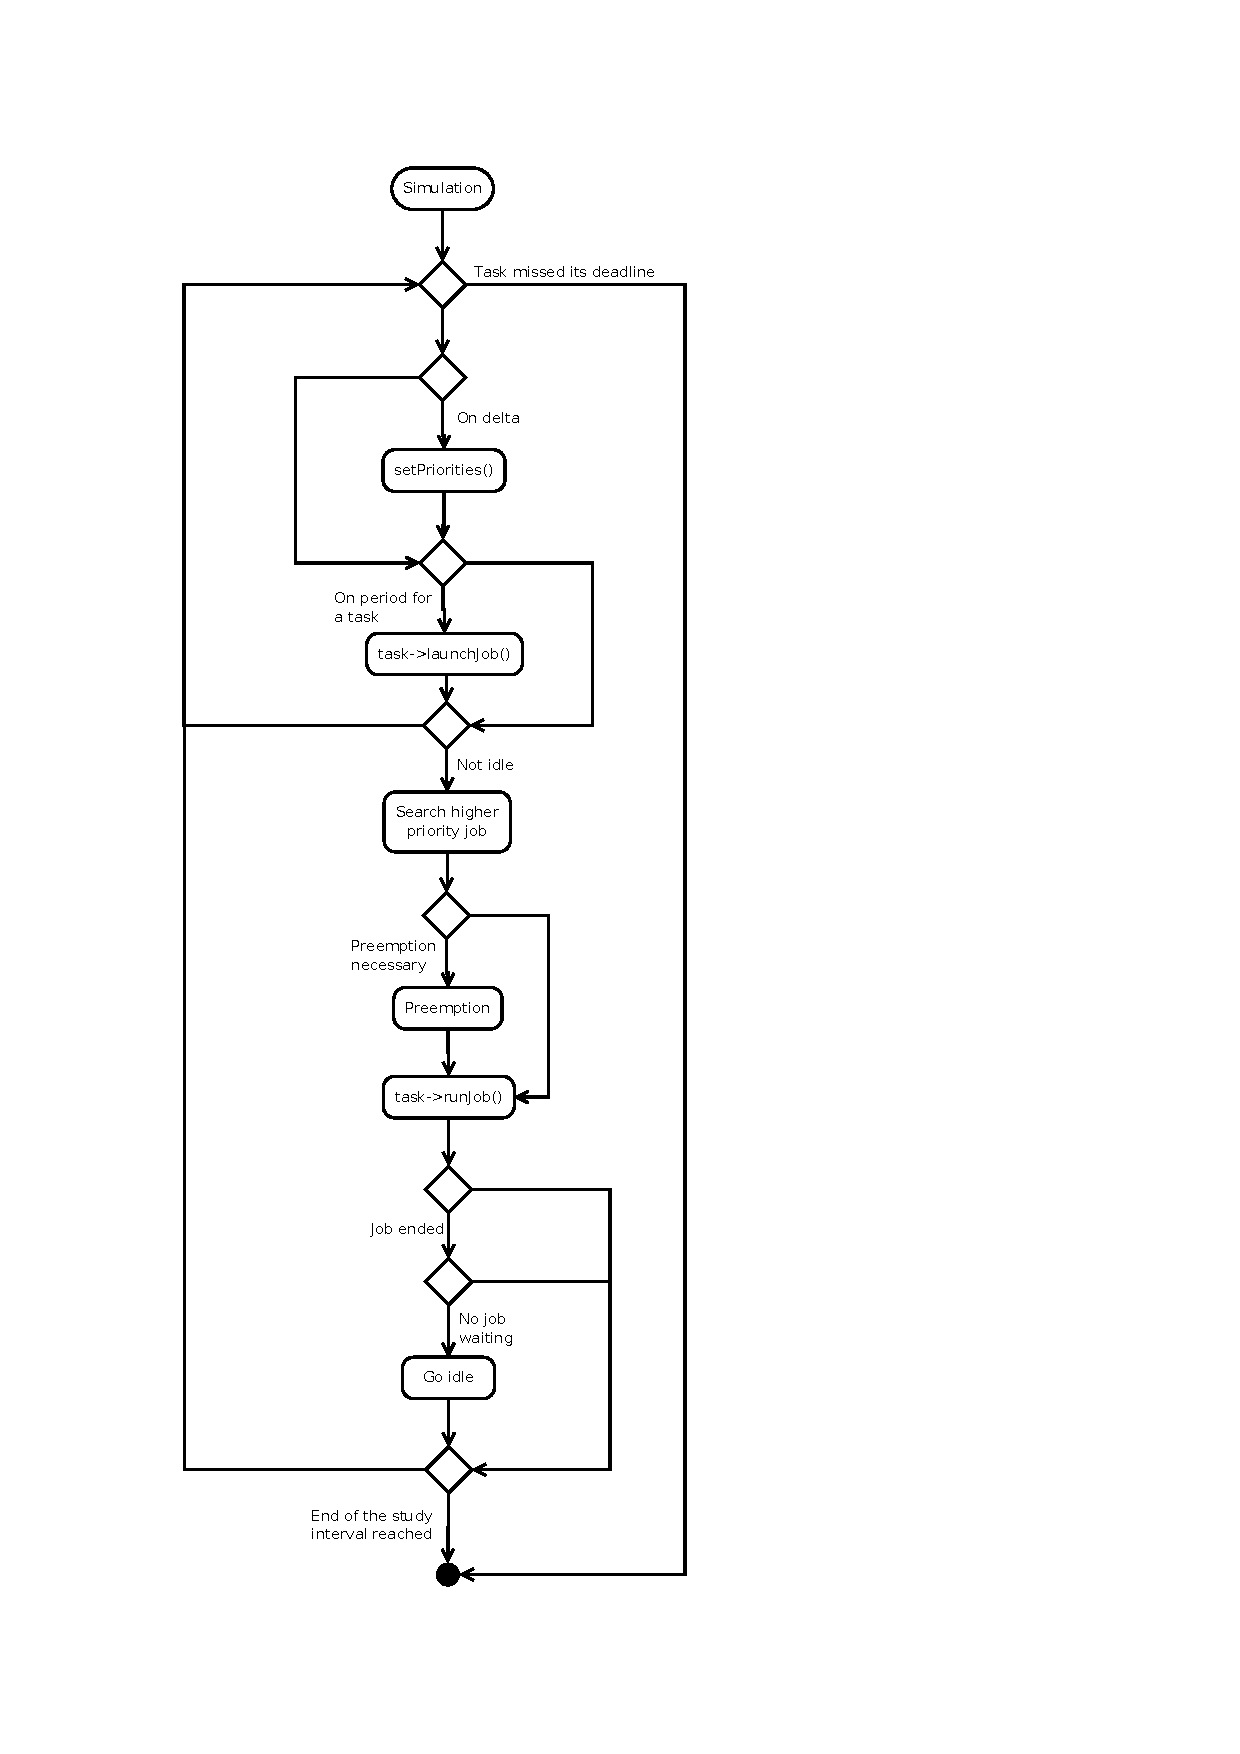
\includegraphics[height=22cm]{StateDiagram}
     
     
    \end{document}


